\chapter{Pharmacometrics}
\section{Additonal PK parameters}
\label{app: add. PK parameters}
%%% Exposure
The exposure of a drug is defined as
\begin{align*}
    \text{exposure} = \int_0^{\infty} C(t) \ dt,
\end{align*}
where $C(t)$ is a given concentration function.

The time when maximum concentration is reached depends on the model. In the one-compartment model without depot (ref), the maximum concentration, $C(t_{\text{max}})$, occurs instantly, i.e. at $t = t_{\text{max}} = 0$, see Figure \ref{fig: Drug Concentration IV}.
% In some cases, it is of interest to prolong the duration of a drug in the body to increase the exposure. An approach to achieve this is to increase the initial amount of drug, $D$, given. This approach may lead to undesired side effects, and is therefore not necessarily preferred. Changing the dosing regimen to constant rate infusion or multiple dosing, can help prolong the duration of the drug.

%%% t and C _max
% It can be important to determine if the concentration exceeds some threshold concentration, or to know what the maximum concentration will be for some dose given the PK parameters. 

\begin{figure}[H]
    \centering
    \begin{minipage}{0.45\textwidth}
        \centering
        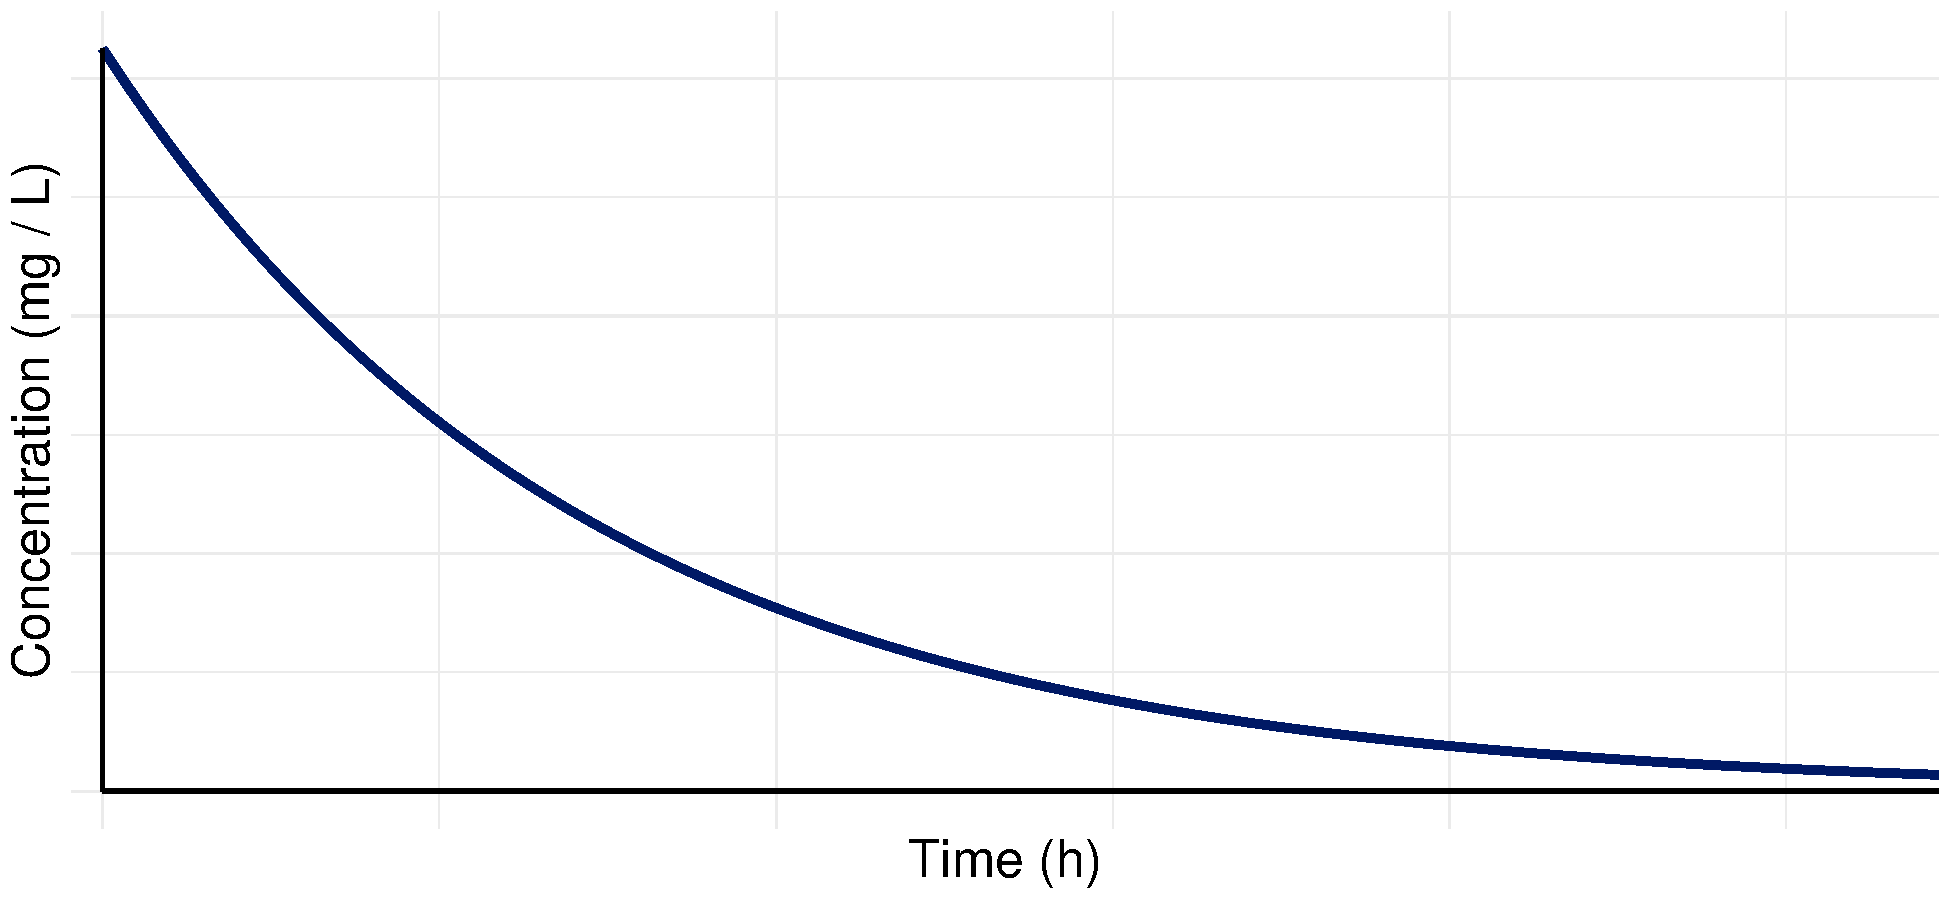
\includegraphics[width=\linewidth]{fig/img/Exposure and Css/Concentration W. IV.pdf}
        \caption{Example of drug concentration for a one-compartment model without depot.}
        \label{fig: Drug Concentration IV}
    \end{minipage}%
    \hfill
    \begin{minipage}{0.45\textwidth}
        \centering
        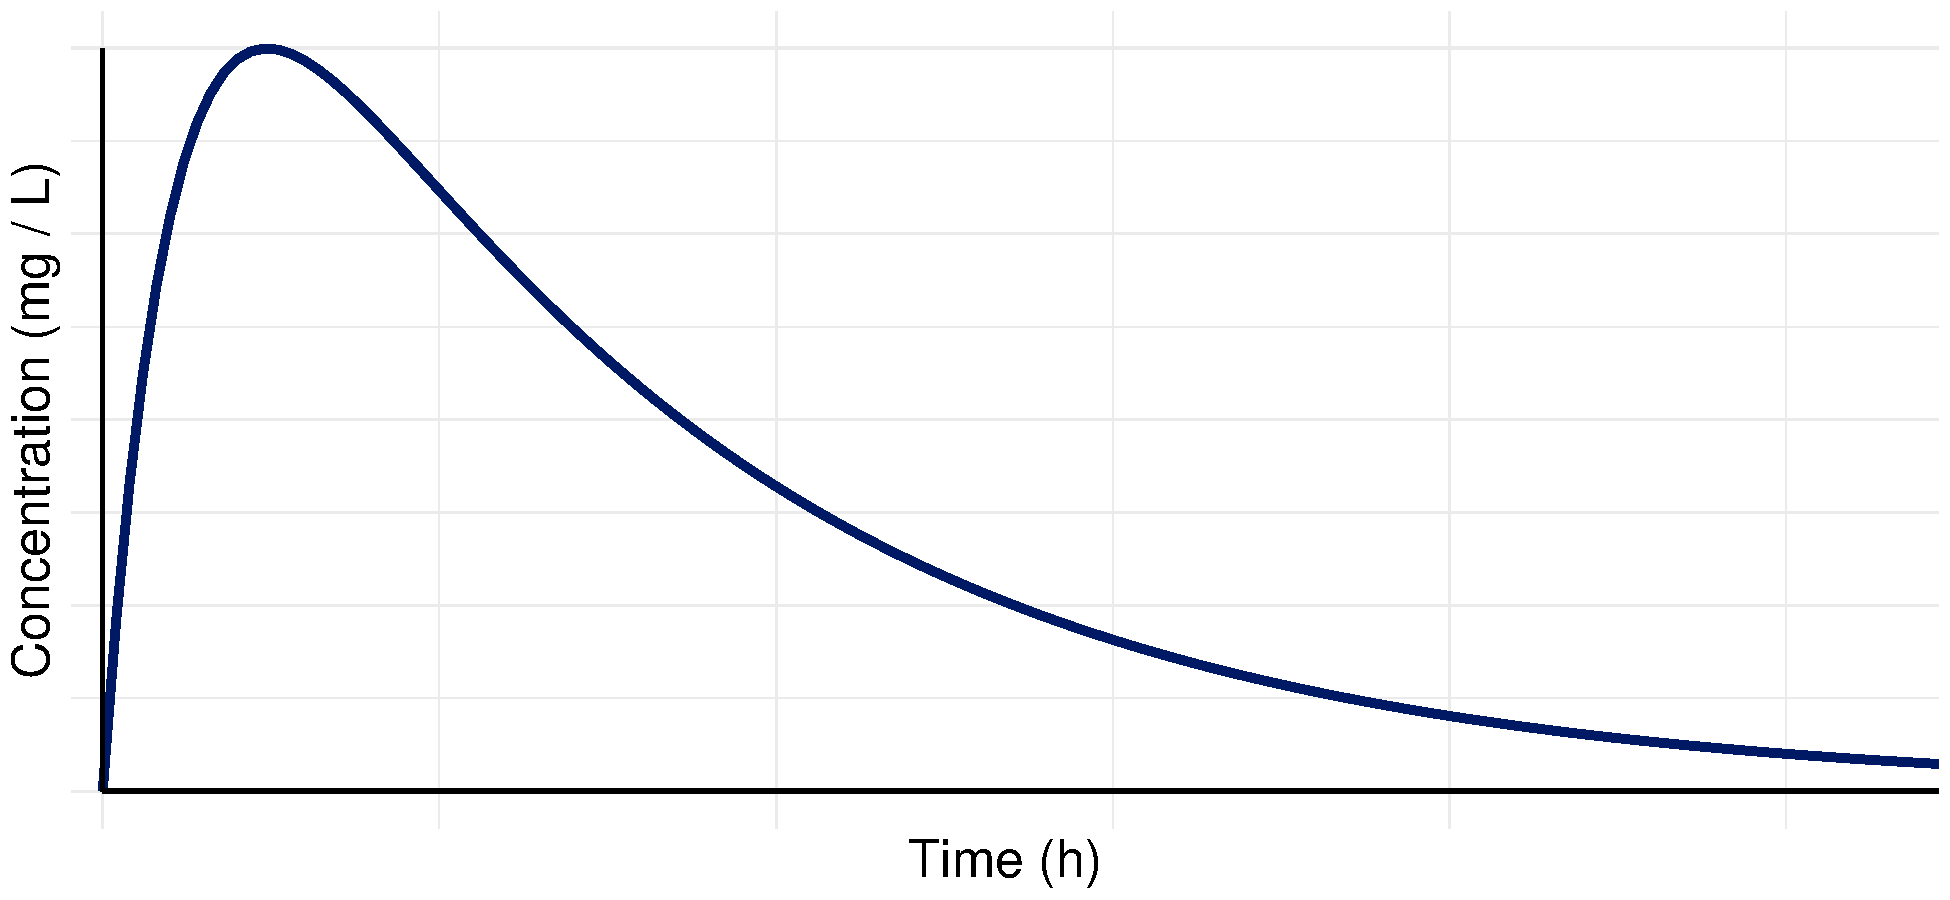
\includegraphics[width=\linewidth]{fig/img/Exposure and Css/Concentration W. Oral.pdf}
        \caption{Example of drug concentration for a one-compartment model with depot.}
        \label{fig: Drug concentration EV}
    \end{minipage}
    \label{fig: Drug concentrations}
\end{figure}

In the one-compartment model with depot (ref), $C(t_{\text{max}})$ occurs at
\begin{align} \label{eq: t_max for one com with absorption}
    t_{\text{max}} = \frac{1}{K_a - K_e} \ln\left(\frac{K_a}{K_e}\right),
\end{align}
and is obtained by setting \eqref{eq: first order kinetic of amount in central com with abs com} equal to zero and solving for $t$, see Figure \ref{fig: Drug concentration EV}. The maximum concentration is then \eqref{eq: sol to first order kinetic of amount in central com with abs com} evaluated in $t_{\text{max}}$.


%%% half-life 
The biological half-life of a drug is the time required for the concentration of a drug in the body to reduce by half. It is given by 
\begin{align}
    t_{1/2} = \frac{\ln(2)}{K_e},
\end{align}
which shows that the half-life only depends on the elimination rate constant $K_e$, meaning it remains constant regardless of the drug concentration. The half-life is obtained by setting \eqref{eq: sol to first order kinetic of amount in one com without abs} equal to $\frac{1}{2}D$ and solve for $t$. 




\section{Other dosage regiments}
\label{app: other dosage regimen}
Consider a one-compartment model with IV administration with constant rate infusion $R_{in}$ (measured in mass per time, e.g. $mg/h$), meaning that a constant amount of drug is injected per unit time. Assuming the rate of infusion is constant, and the drug elimination follows first order kinetics, the mass balance equation for the central compartment during the time of infusion is given by
\begin{align} \label{eq: Constant infusion rate}
    \Dif{A_{central}(t)}=R_{in}-K_e*A_{central}(t), 
\end{align}
where $R_{in}$ is a constant indicating the amount of drug injected into the central compartment per unit time. When the infusion of drug stops, i.e. $R_{in}=0$, the mass balance equation simply describes drug elimination following first order kinetics. The solution to \eqref{eq: Constant infusion rate} is divided by $V_d$ to obtain the solution expressed in terms of concentration,
\begin{align*}
    C_{central}(t) = \frac{R_{in}}{Cl}\left(1-\exp\left(-K_e * t\right)\right).
\end{align*}

Figure \ref{fig: IN and MD} shows an example of concentration of a drug administered IV with constant rate infusion. This illustrates that the concentration increases until the elimination rate equals the infusion rate, and a steady state is reached. This occurs as the infusion rate is constant, and the elimination rate is proportional to the drug concentration. The concentration at which steady state occurs is obtained by setting \eqref{eq: Constant infusion rate} equal to zero and using the relations \eqref{eq: Concentration} and \eqref{eq: elimination rate constant},
\begin{align*}
    R_{in} = K_e * A_{central}(t_{ss}) \Longrightarrow R_{in} = \frac{Cl}{V_d}A_{central}(t_{ss}) \Longrightarrow
    C(t_{ss}) = \frac{R_{in}}{Cl},
\end{align*}
where $C(t_{ss})$ denotes the steady state concentration at time $t_{ss}$, where $t_{ss}$ denotes time points for which \eqref{eq: Constant infusion rate} equals $0$. This implies that the steady state concentration is known given the constant infusion rate and clearance.

%%% Multiple dosing
Consider a one-compartment model with EV administration and $N$ doses given at the same time interval $\tau$ between every dose. This scenario has same method of administration and number of compartments as the scenario for the mass balance equation \eqref{eq: first order kinetic of amount in central com with abs com}, but the dosing regimen is different. Assuming the absorption follows first order kinetics, the concentration for multiple dosing is the sum of the remaining concentration of each EV administered dose received, 
\begin{align*}
    C(t) = \sum^{N-1}_{n=0} C_{single}(t-n*\tau),
\end{align*}
where $C_{single}$ is \eqref{eq: sol to first order kinetic of amount in central com with abs com} divided by $V_d$.

Multiple dosing can be interpreted as an approximation of constant rate infusion, where the administration is EV instead of IV, as IV administration is not always possible. The multiple dosing is related to the infusion rate by
\begin{align*}
    R_{in} = \frac{F * D}{\tau}.
\end{align*}

An example of concentration of a drug administered EV with multiple dosing can be seen in Figure \ref{fig: IN and MD}.
\begin{figure}[H]
    \centering
    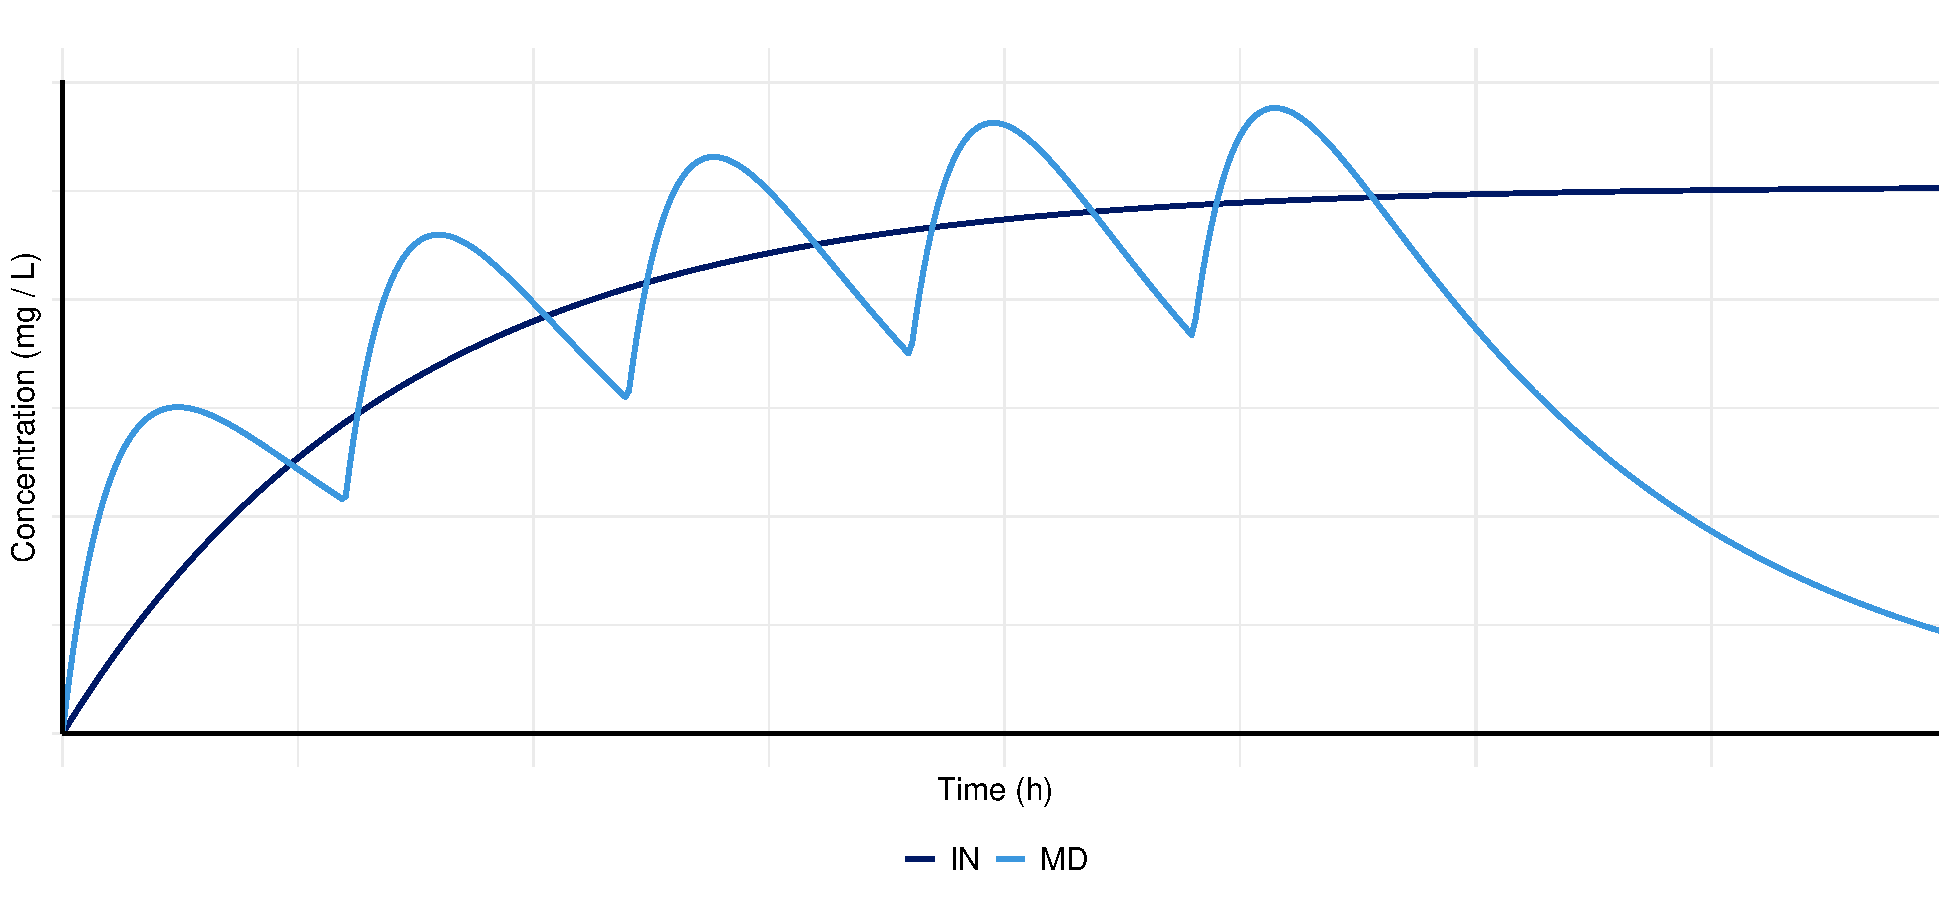
\includegraphics[width=0.9\linewidth]{fig/img/Exposure and Css/3hoursDosing.pdf}
    \caption{Example of drug concentration obtained with constant rate infusion and multiple dosing.}
    \label{fig: IN and MD}
\end{figure}



\section{Effect derivations}


The expression is obtained by 
From \eqref{eq: steady state PD}, it can be derived that
\begin{align} \label{eq: Steady state derivation}
    \frac{[R][M]}{[MR]} = K_d \implies \frac{[MR]}{R_{tot}} = \frac{[M]}{[M] + K_d},
\end{align}
where $k_d = \frac{k_{-1}}{k_1}$ is the disassociation constant.
The first equation in \eqref{eq: Steady state derivation} is obtained directly from \eqref{eq: steady state PD}, and the second equation in \eqref{eq: Steady state derivation} is derived by substituting $[R]$ in the first equation with $([R_{tot}] - [MR])$. 

To derive the expression in \eqref{eq: Steady state derivation} in terms of effect, the quantities $[MR]$ and $[R_{tot}]$ are substituted with the relationships established in \eqref{eq: effect formalisation} and \eqref{eq: effect formalisation2}, such that
\begin{align} \label{eq: Effect and concentration}
    \frac{E/\varphi}{E_{\text{max}}/\varphi} = \frac{[M]}{[M] + K_d} \implies E = \frac{E_{\text{max}}[M]}{[M] + K_d}.
\end{align}
The amount of unbounded drug molecules, $[M]$, is interpreted as the drug's concentration.


\section{Table of parameters}

\begin{table}[h!]
    \centering
    \renewcommand{\arraystretch}{1.5}
    \begin{tabular}{|p{3.4cm}|p{1.4 cm}|p{8.8cm}|}
        \hline
        \textbf{Parameter} & \textbf{Unit} & \textbf{Description} \\
        \hline
        $F$ (bioavailability) & unitless & The fraction of the administered dose that reaches the systemic circulation. \\
        \hline
        $V$ (volume of distribution) & $\text{volume}$ & Relation between total amount of drug in the body and the plasma concentration of the drug. \\
        \hline
        $Cl$ (clearance) & $\tfrac{\text{volume}}{\text{time}}$ & The volume of plasma cleared of drug per time. \\
        \hline
        $k_a$ (absorption rate constant) & $\text{time}^{-1}$ & The rate at which the drug moves from the site of administration into the systemic circulation. \\
        \hline
        $k_e$ (elimination rate constant) & $\text{time}^{-1}$ & The rate at which a drug is eliminated from the body.\\
        \hline
        $k_{12}$, $k_{21}$ (exchange rate constants) & $\text{time}^{-1}$ & The rate at which the drug distributes between various tissues of the body. \\
        \hline
    \end{tabular}
    \caption{Description of PK parameters with units of measure.}
    \label{tab: pharmacokinetic parameters summary}
\end{table}